\chapter{Welcome to the Galaxy}

Looking up on a clear, dark night, our eyes are able to discern a
luminous band stretching across the sky.  Observe it with  
binoculars or a small telescope and you will discover, like Galileo in
1609, that it is made up of a myriad of stars.  This is the {\bf Milky
Way}: our own Galaxy, as it appears from Earth.  It contains about a  
hundred billions of stars, and our Sun is just one of them. There are
many other galaxies in the universe.

It took astronomers a long time to figure out what our Galaxy really
looks like.  One would like to be able to embark on a spaceship and
see the Galaxy from outside.  Unfortunately, traveling in and around
the Galaxy is (and will always be) out of the question because of the huge
distances.  We are condemned to observe the Galaxy from the vicinity
of the Sun.  In addition, some areas of the Milky Way appear darker
than others; this is because they are obscured by large amounts of
interstellar dust, and we can't even see the stars that lie behind the
dust clouds.

Observations of other galaxies and of our own, both with optical and
radio telescopes, have helped unveil the structure of our Galaxy.
Now, astronomers think that they have a good knowledge of how the
stars and the gas are distributed.  Our Galaxy seems to look like a
thin disk of stars and gas, which are distributed in a spiral pattern.

But a new mystery has arisen: that of the so-called {\bf dark matter}.
Most of the mass of our Galaxy seems to be in the form of dark matter,
a mysterious component that has, so far, escaped all means of
identification.  Its existence has been inferred only indirectly. Imagine a
couple of dancers, in a dark room. The man is black, dressed in black
clothes, and the woman wears a fluorescent dress. You can't see the
man. But from the motion of the woman dancer, you can infer his
presence: somebody must be holding onto her, otherwise, with such
speed, she would simply fly away!  Similarly, the stars and the gas in
our Galaxy rotate {\em too fast}, compared to the amount of mass
observed. There must therefore be {\em more matter}, invisible to our eyes
and to the most sensitive instruments, but which, through the force of
gravity, holds the stars together in our Galaxy and prevents them from
flying away. The key argument in favor of the existence of dark
matter comes from the measured velocities in the outer part of our
Galaxy.  Radio measurements of the type discussed here have played an
important role in revealing the presence of dark matter in the
Galaxy. But what dark matter really is remains an open question.

\vfill\eject
\section{Where are we in the Milky Way?}
\subsection{Galactic longitude and latitude}

Our star, the Sun, is located in the outer part of the Galaxy, at a distance of
about 8.5~kpc\footnote{1 kpc = 1 kiloparsec = 10$^3$ pc; 1 parallax-second
(parsec, pc) = 3.086$\cdot 10^{16}$~m.  A parsec is the distance from which the
radius of Earth's orbit subtends an angle of $1''$ (1~arcsec).} (about
25~000~light years\footnote{1 light year (ly) = 9.4605$\cdot 10^{15}$~m}) from
the Galactic center.  Most of the stars and the gas lie in a thin disk and
rotate around the Galactic center.  The Sun has a circular speed of about
220~km/s, and performs a full revolution around the center of the Galaxy in
about 240 million years.

To describe the position of a star or a gas cloud in the Galaxy, it is
convenient to use the so-called {\bf Galactic coordinate system}, $(l,b)$,
where $l$ is the Galactic longitude and $b$ the Galactic latitude (see
Fig.~\ref{figdisc} and Fig.~\ref{figmwsketch}).  The Galactic coordinate system
is centered on the Sun.  $b=0$ corresponds to the Galactic plane. The direction
$b=90\deg$ is called the North Galactic Pole. The longitude $l$ is measured
{\it counterclockwise} from the direction from the Sun toward the Galactic
center.  The Galactic center thus has the coordinates ($l=0,b=0$).  There is,
in fact, something very special at the Galactic center: a very large
concentration of mass in the form of a black hole containing approximately
three million times the mass of the Sun.  Surrounding it is a brilliant source
of radio waves and X-rays called Sagittarius~A*. 


\begin{figure}[ht]
\begin{center}
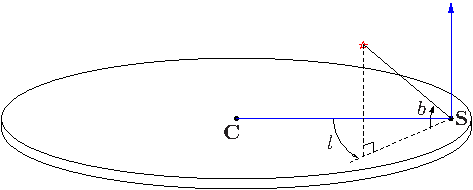
\includegraphics[width=8cm]{../figures/galdisc.pdf}
\end{center}
\caption{Illustration of the Galactic coordinate system, with longitude ($l$) and latitude ($b$). 
{\bf C} indicates the location of the Galactic center, {\bf S} the location of the Sun.}
\label{figdisc}
\end{figure} 

\begin{figure}[ht]
\begin{center}
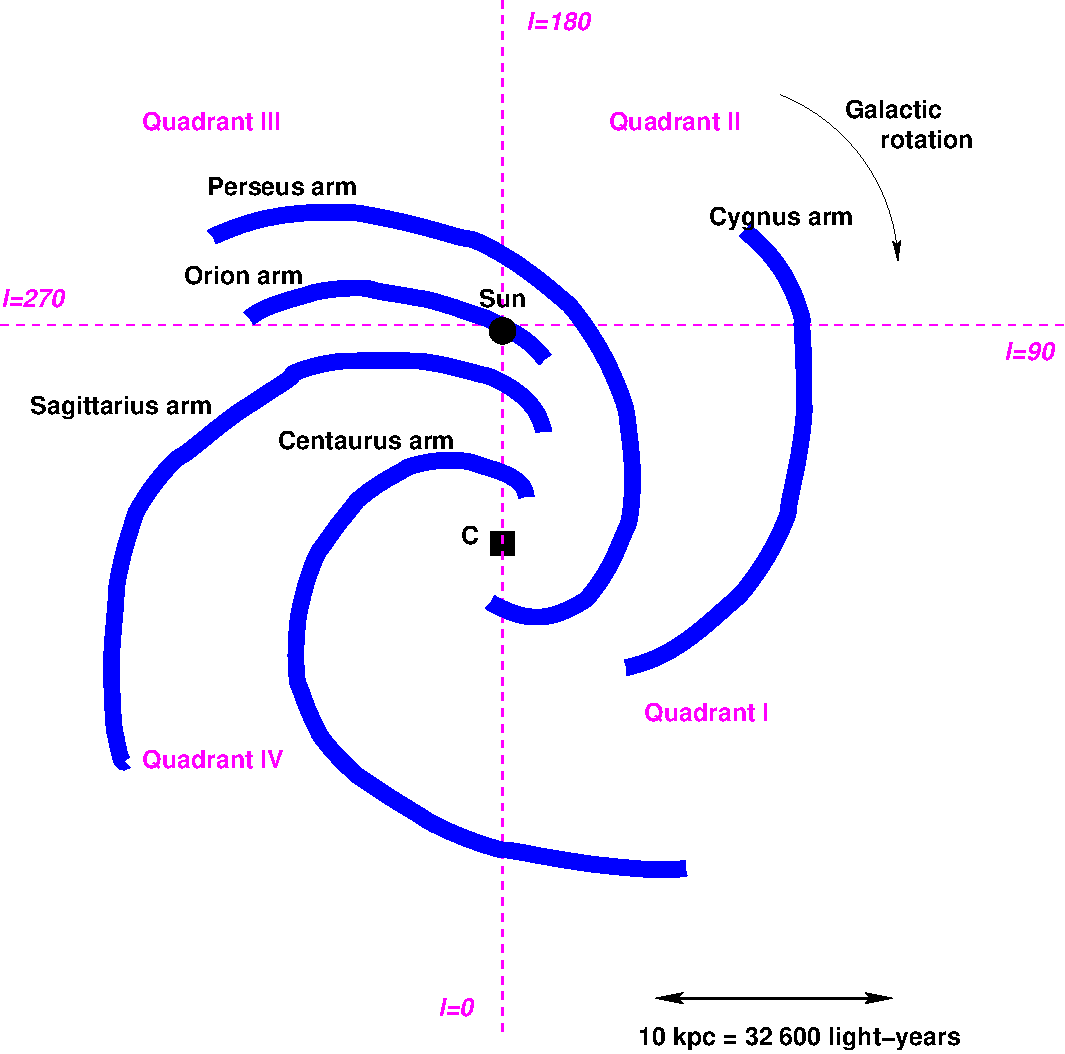
\includegraphics[width=10cm]{../figures/mwsketch.pdf}
\end{center}
\caption{Sketch of the spiral structure of the Galaxy. 
{\bf C} indicates the location of the Galactic center. 
The
approximate locations of the main spiral arms are shown. The
locations of the four quadrants are indicated.}
\label{figmwsketch}
\end{figure}  


The Galaxy has been divided into four quadrants, labeled by 
roman numbers: 
\bigskip
\begin{displaymath}
\begin{array}{lc}
\hbox{Quadrant {\sc I}} 	&0\deg < l < 90\deg	\\
\hbox{Quadrant ${\rm II}$} 	&90\deg < l < 180\deg	\\
\hbox{Quadrant ${\rm III}$} 	&180\deg < l < 270\deg	\\
\hbox{Quadrant ${\rm IV}$} 	&270\deg < l < 360\deg 
\end{array}
\end{displaymath}
\bigskip

Quadrants II and III contain material lying  
at galacto-centric radii which are always {\it larger} than the Solar
radius (the radius of the orbit of the Sun around the Galactic center).

In Quadrant~I and IV one observes mainly the inner part of
our Galaxy. 


\subsection{Notations}

\begin{figure}[ht]
\begin{center}
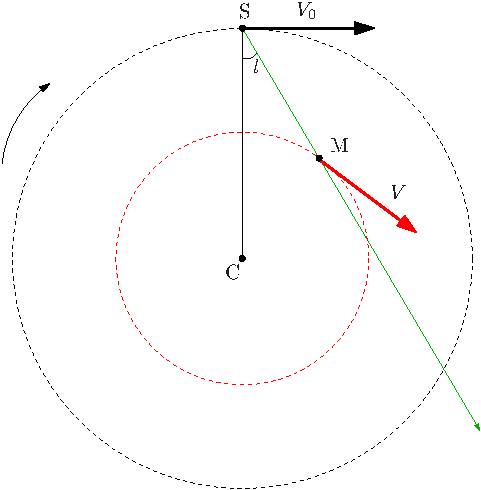
\includegraphics[width=7cm]{../figures/suncloud.pdf}
\end{center}
\caption{Geometry of the Galaxy. {\bf C} is the location of the Galactic center, 
{\bf S} that of the Sun, {\bf M} that of a gas cloud that we want to observe. 
The SM line is the line-of-sight. The arrow on an arc indicates the direction 
of rotation of the Galaxy. The arrows on line segments indicate the
velocity of the Sun ($V_0$) and the gas cloud ($V$).}
\label{figgeom}
\end{figure}  

Let us first define some notations. 
Some of them are illustrated in Figs.~\ref{figgeom} and \ref{galgeom}.

\begin{displaymath}
\begin{array}{ll}
V_0 	&\hbox{Sun's velocity around the Galactic center} 	\\
        & (220 \hbox{ km/s})					\\
R_0	&\hbox{Distance of the Sun to the Galactic center} 	\\
        & (8.5 \hbox{ kpc}) 					\\
l	&\hbox{Galactic longitude}				\\
V	&\hbox{Velocity of a cloud of gas}			\\
R	&\hbox{Cloud's distance to the Galactic center}		\\
r	&\hbox{Cloud's distance to the Sun}
\end{array}
\end{displaymath}


\section{Looking for hydrogen}

Most of the gas in the Galaxy is atomic hydrogen (H). 
H is the simplest atom: it has only one proton and one electron. 
Atomic hydrogen emits a radio 
line at a wavelength $\lambda= 21$~cm (or a frequency $f=c/\lambda=1420$~MHz,
where $c\simeq 300 000\, {\rm km/s}$ is the speed of light).  
This is the signal we want to detect. 

\begin{equation}
\color{red}{\boxed{
\lambda = 21 \, {\rm cm}
\Rightarrow f=c/\lambda = 1420 \, {\rm MHz}}}
\end{equation}

This spectral line is produced when the electron's spin flips
from being parallel to being antiparallel with the proton's spin, 
bringing the atom to a lower energy state (see Fig.~\ref{fighyperfin}).  
Although this happens spontaneously only about once every ten million years for a
given hydrogen atom, the enormous quantity of hydrogen in the Milky
Way makes the 21~cm line detectable.  The line was predicted by the Dutch
astronomer H.C. van de Hulst in 1945, who determined its frequency theoretically. 
The line was observed for the first time
in 1951 by three groups, in the U.S.A., in the Netherlands and in
Australia (see Appendix~\ref{app-history}).

\begin{figure}[ht]
\begin{center}
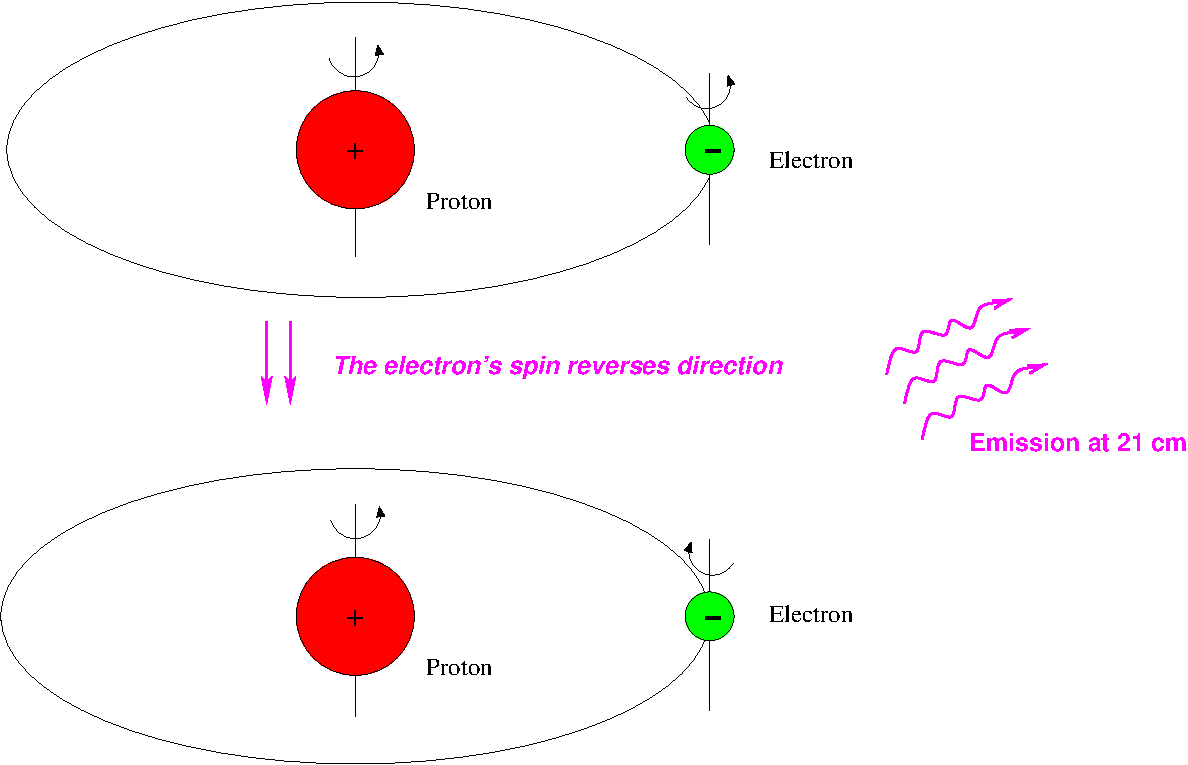
\includegraphics[width=10cm]{../figures/hyperfine.pdf}
\end{center}
\caption{Illustration of the 21~cm transition of the hydrogen atom, 
caused by the energy change when the electron's spin changes from 
parallel with the proton's spin to antiparallel.}
\label{fighyperfin}
\end{figure}  


\section{The Doppler effect}

By observing radio emission from hydrogen, we can also learn about the
motion of the hydrogen gas clouds in our Galaxy. 
Indeed, it is possible to relate the observed {\em frequency} of the
signal to the {\em velocity of the emitting gas}, thanks to the
so-called {\em Doppler effect}.

This effect, named after the Austrian physicist Christian Johann
Doppler (1803--1853), is present in our everyday life; for example if
you are standing still in the street and an ambulance {\em approaches} you,
it appears as if the pitch of the ambulance's siren
{\em increases}. Similarily, when the ambulance {\em is receding}, the pitch of
the siren {\em decreases}. Because sound waves travel through a medium (the
air), when the ambulance is approaching the waves will be 'squeezed'
together by the forward motion. Shorter wavelengths mean higher
frequency, and thus the pitch of the siren increases.

There is another mechanism we need to understand.  
One of the greatest scientific achievements of the 20th
century was the theory of Special Relativity, presented by Albert
Einstein in 1905. A postulate of the theory is
that the speed of light is constant. We may use a simple example: a
person stands by the road and watches a car drive towards her at
a speed of 90 km/h. The driver throws a ball in the direction of the
car at a speed of 200 km/h. The person standing by the road will
observe the ball coming towards her at the speed of 90+200=290
km/s. Imagine that the driver instead would put out a flashlight that
emits light at the speed of light ($c$), and the person by the road
would have a way of measuring the speed of the lightbeam coming
towards her, the velocity of the beam would not be 90~km/h~$+ c$, 
but only $c$. This is because the speed of light is constant in
all intertial frames, that is, in non-accelerating frames.
Einstein showed how the relative motions of the ball and of light could be
consistent with each other: the former is the low-speed approximation of the
latter. 

We must use the Doppler effect to relate frequency to velocity.
A rather long derivation shows that

\begin{equation}
\color{red}{\boxed{
\frac{\Delta f}{f_0}=-\frac{v}{c}
}}
\end{equation}

where 

\begin{displaymath}
\begin{array}{ll}
\Delta f=f-f_0	&\hbox{is the frequency shift}, 	\\
f		&\hbox{is the observed frequency} 	\\
f_0		&\hbox{is
the rest frequency of the line we are observing}	\\
v		&\hbox{is the velocity, $> 0$ if the object is
receding,}						\\
		&\hbox{$< 0$ if it is approaching.}
\end{array}
\end{displaymath}

When we want to observe the $\lambda$21~cm line of hydrogen along a Galactic
longitude, we tune the receiver of our radio telescope to a frequency band near
the exact frequency of the hydrogen line. This will allow us to find hydrogen
gas with different velocities that emit at the frequency of 1420~MHz (the rest
frequency of the radio line), although the frequency is shifted up or down when
it reaches us, depending on whether the gas cloud that we observe is
approaching us or receding from us. 

